\documentclass{beamer}

\usepackage{../packages/packages_mathalea}
\input{../competences/competences_latex.tex}
\usepackage{fontawesome}

\pgfplotsset{compat=1.18}

\begin{document}

\begin{frame}{\GetCompetence{Fonc10}}
	\begin{itemize}
		\item Déterminer une équation cartésienne de la droite $(d1)$ passant par les points $A(1; -2)$ et $B(-3;-4)$.
		\item Déterminer l'expression réduite de la droite $(d2)$ représentée ci-dessous.
	\end{itemize}
	\begin{minipage}[t]{0.65\textwidth}{
	\vspace{0pt}
\begin{center}
	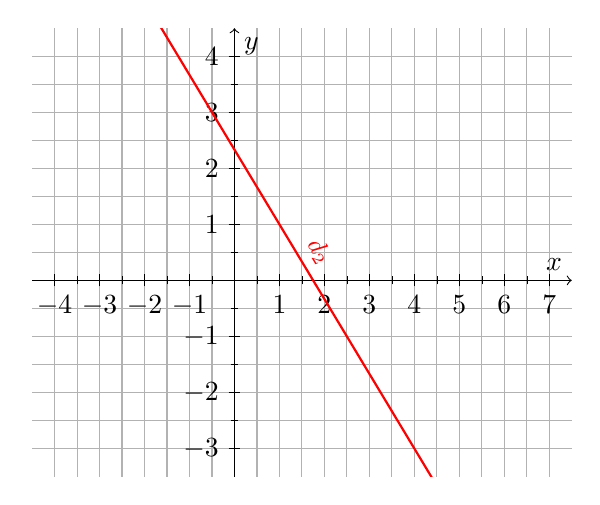
\begin{tikzpicture}[scale=1]
    % Define axis
    \begin{axis}[
        axis lines=middle,
        grid=both,
        minor tick num=1,
        xlabel={$x$},
        ylabel={$y$},
        xmin=-4.5, xmax=7.5,
        ymin=-3.5, ymax=4.5,
        xtick={-4,-3,-2,-1,0,1,2,3,4,5,6,7},
        ytick={-3,-2,-1,0,1,2,3,4},
        axis line style={->},
        tick style={black},
        label style={font=\bfseries},
        grid style={black!30}
    ]
        % Line d1
        \addplot[domain=-4:7, thick, red] { - 4/3*x+7/3} node[pos=0.5, above, sloped] {\small $d_2$};
    \end{axis}
\end{tikzpicture}
\end{center}

	
	}
	\end{minipage}
     \onslide<2->{	
	\begin{minipage}[t]{0.3\textwidth}{
	\vspace{0pt}
	Réponses : 
	\begin{itemize}
		\item[$(d1)$]: $2y-x+5=0$
		\item[ $(d2)$]: $y=-\dfrac{4}{3}x+\dfrac{7}{3}$
	\end{itemize}
	}
\end{minipage}}
\end{frame}
\end{document}
